\newpage

\chapter{Requirements and Analysis}
In response to the pressing need for seamless healthcare monitoring, this project introduces VitalMonitor, a centralized system designed to enhance real-time monitoring of healthcare professional (HCP) vitals. This innovative IoTaaS platform comprises two key components: the Smart Patch, a wearable IoT device for vital sensing, and a comprehensive dashboard for monitoring and managing healthcare professionals. VitalMonitor not only simplifies access to vital health metrics but also integrates these functionalities into a user-friendly platform, minimizing the technological burden on healthcare organizations and easily integrate into their exisiting workflow. The chapter covers on the required features of the system, risk analysis and an evaluation system for VitalMonitor is introduced.

\section{Parameters for Healthcare Monitoring}

To effectively monitor stress and fatigue levels in real-time, the Smart Patch will utilize two key physiological parameters. The selection of these parameters is crucial to ensure accurate and actionable health insights for healthcare professionals (HCPs) working in demanding environments. Identifying relevant parameters is vital to the Smart Patch's efficacy. The VitalMonitor project focuses specifically on stress and fatigue levels because of their significant impact on healthcare professionals. A range of physiological and psychological indicators were considered, but only those with high relevance and monitoring feasibility were selected. \\ 

\noindent A comparative analysis of potential monitoring parameters was conducted based on relevance to stress and fatigue and the feasibility of non-intrusive monitoring. Table \ref{tab:health_parameters} presents the results of this analysis. Based on this analysis, Heart Rate Variability (HRV) and Body Temperature are identified as the most relevant parameters for monitoring stress and fatigue levels. These parameters offer the advantage of continuous, non-intrusive monitoring through the Smart Patch. \\ \\ \\

\begin{table}[h!]
\centering 
\begin{tabularx}{\textwidth}{|X|X|X|}
\hline 
\textbf{Parameter} & \textbf{Relevance to Stress/Fatigue} & \textbf{Monitoring Feasibility} \\ 
\hline Heart Rate Variability (HRV) & High & High \\ 
\hline Body Temperature & Moderate & High \\ 
\hline Blood Pressure & High & Moderate \\ 
\hline Galvanic Skin Response & High & Moderate \\ 
\hline Cortisol Levels & High & Low \\ 
\hline
\end{tabularx}
\caption{Comparison of Health Monitoring Parameters}
\label{tab:health_parameters}
\end{table}



\noindent While HRV provides detailed insights into an individual's stress and fatigue levels, it is challenging to calculate due to the following reasons:
\begin{itemize}
    \item  \textbf{Sensor Accuracy:} HRV requires highly accurate sensors to capture subtle variations in heart rhythm.
    \item  \textbf{Noise Interference:} Movement and other physiological signals can interfere with the accuracy of HRV measurements.
    \item  \textbf{Data Processing:} Advanced algorithms are required to accurately interpret HRV data.
\end{itemize}

\noindent Therefore, for simplicity and ease of implementation, Heart Rate (beats per minute) will be used instead of HRV. Although this approach provides slightly less nuanced information, it still allows effective monitoring of stress and fatigue levels.


\section{VitalMonitor: System Description}
VitalMonitor marks a significant advancement in healthcare technology by prioritizing the well-being of HCPs in high-stress environments. This system includes the Smart Patch, a discrete, non-intrusive wearable device tailored for healthcare settings, and a web-based dashboard that facilitates real-time data analysis and monitoring. The goal is to deliver actionable insights into HCP health, enabling timely interventions to alleviate stress and fatigue, and thereby enhancing patient care and safety. \\ 

\noindent VitalMonitor will provide passive health monitoring of HCPs to the organization admins. Passive monitoring refers to the process of collecting data from individuals without requiring their active participation or input. In healthcare, passive monitoring typically involves the use of sensors or other technology to continuously gather data on various physiological parameters. This doesn't require the need for individuals to perform any specific actions or interactions. \\ 

Figure \ref{fig:sys-desc} visually represents how VitalMonitor will work all in all and how different components of VitalMonitor will interact and work together.

\begin{figure}
    \centering
    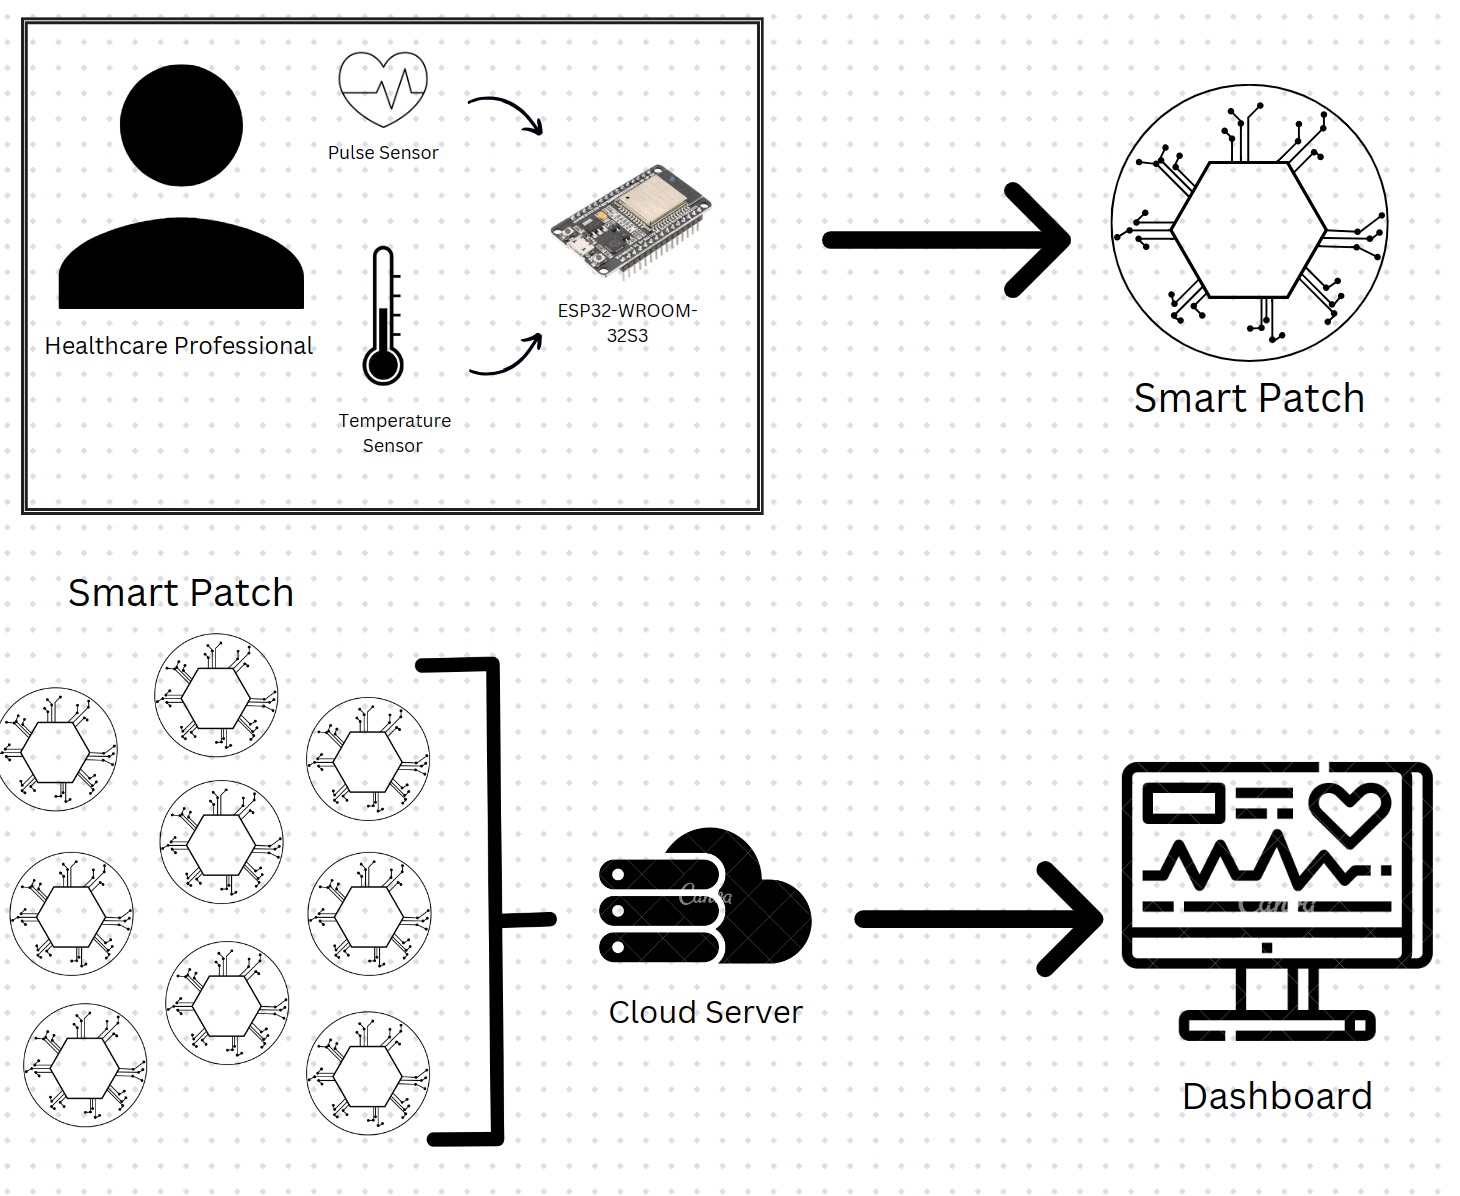
\includegraphics[width=0.9\linewidth]{images/sys-desc.png}
    \caption{VitalMonitor: High-level working diagram}
    \label{fig:sys-desc}
\end{figure}

\subsection{Smart Patch}
The Smart Patch is a non-intrusive wearable IoT device which will be designed to monitor the health and well-being of healthcare professionals in high-stress environments. This innovative IoT device aims to address the limitations of existing wearable technologies, particularly the restrictions on wearing smartwatches in healthcare settings. \\ 

 \noindent While stress and fatigue are complex and multifaceted, heart rate and body temperature serve as surrogate markers that can be effectively measured in real-time. The integration of these parameters into the Smart Patch enables continuous monitoring, offering valuable insights into HCPs’ health and well-being. By focusing on these indicators, the Smart Patch aims to provide actionable data that empowers healthcare institutions to proactively address stress and fatigue, ultimately enhancing the overall quality of care in high-stress environments.
 
 \subsubsection{Device Placement}
The placement of the Smart Patch is crucial to ensure reliable vital sign measurements while minimizing interference with healthcare professionals' tasks. Research in clinical physiology suggests that the ear lobe is an ideal site for accurate and consistent heart rate measurement due to its rich vascular supply and proximity to the surface, which makes it less susceptible to external noise interference and movement artifacts. Additionally, the area behind the ear is well-suited for measuring body temperature, as this region is less exposed to ambient temperature variations than other body surfaces, providing a more accurate reading of core temperature.\\

\noindent Moreover, the ear region provides an advantageous, non-intrusive position where the device is unlikely to interfere with daily tasks. This ensures the comfort and continuous monitoring of HCPs. Figure \ref{fig:device-placement} illustrates the optimal placement of the Smart Patch, highlighting the exact positions on the ear lobe (for heart rate measurement) and behind the ear (for temperature sensing) in red.\\

\noindent By positioning the Smart Patch in these locations, the system can reliably collect data while ensuring that healthcare professionals can work without distraction or discomfort.

 \begin{figure}[h!]
     \centering
     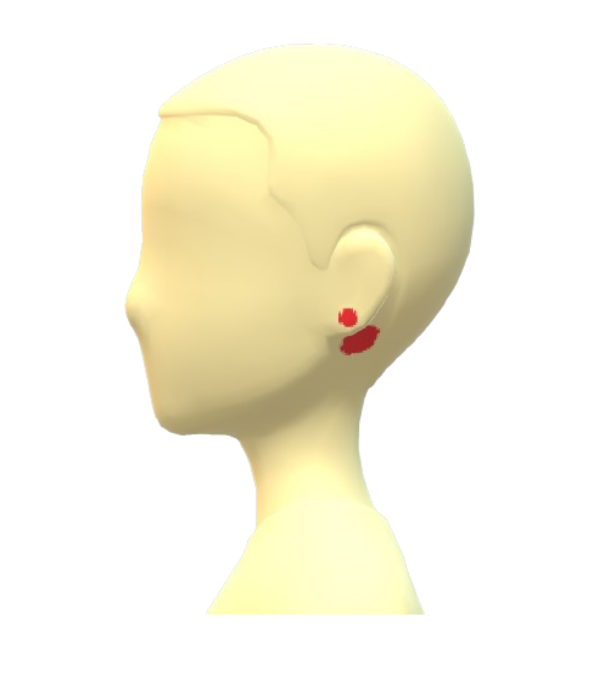
\includegraphics[width=0.3\linewidth]{images/device-placement.png}
     \caption{Device Placement}
     \label{fig:device-placement}
 \end{figure}

\subsection{Dashboard}
 To facilitate real-time monitoring, a web dashboard will be made where the institutions can track the vitals of all the HCPs working at that time using the data being collected by smart patch in real-time. It will present options to get alerts when an HCP’s vital signs go beyond the threshold. Overall,  the dashboard serves as a central hub for visualizing and interpreting the data collected by the smart patch, facilitating informed decision-making and proactive measures to support the health and well-being of HCPs in high-stress environments. \\ \\

\noindent Agile methodology of the Software Development Lifecycle (SDLC) (refer to \textbf{Appendix \ref{app:agile}}) will be used for creating both the Smart Patch and the dashboard.
  
\section{Requirements of the system}
 Both the Smart Patch and the Dashboard boast a set of functional and non-functional requirements meticulously designed to ensure seamless real-time monitoring by healthcare professionals (HCPs). These are categorized as follows: 

  \begin{itemize}
        \item \textbf{User Stories} \\ 
        User stories capture the requirements from the user's perspective, providing insights into their needs. The stories are grouped by user roles. These user stories, along with their priorities, are presented in Table~\ref{tab:longtable}.
        
        \item \textbf{Functional Features} \\
    Functional features represent the capabilities and behaviours of a system that directly contribute to its primary purpose and functionality. These features are concerned with what the system does and how well it performs its intended tasks. 

        \item \textbf{Non-Functional Features} \\
    Non-functional features, on the other hand, are characteristics of a system that do not directly relate to its specific functionalities but rather focus on how well the system performs its functions. 
    
    \end{itemize}
 
 Additionally, they are prioritized using the MoSCoW prioritization framework into Must-Have, Should-Have, Could-Have, and Won’t-Have categories, as illustrated in the Tables \ref{table:functional-sp-db}-\ref{table:non-functional-sp-db}. Key to priority framework is given in Table \ref{tab:key-to-features}.
 

 \begin{table}[h!]
        \centering
        \begin{tabularx}{\textwidth}{|p{3cm}|X|}
            \hline
             \textbf{Category} 
             & \textbf{Description} \\ \hline

             \textbf{Must-Have} 
             & This category consists of features that are “must” for the system. They represent non-negotiable needs for the system.  
             \\ \hline

             \textbf{Should-Have} 
             & 	They are essential for the system, but they are not vital. If left out, the system still functions. However, the features  may add significant value. 
             \\ \hline

             \textbf{Could-Have} 
             & These features are not necessary to the core function of the system. 
             \\ \hline

             \textbf{Won't-Have} 
             & This category contains features which will not be included in a specific release, time frame or prioritised in the future. Their absence is not detrimental to the functionality of the final product.
             \\ \hline 
        \end{tabularx}
        \caption{Key to features}
        \label{tab:key-to-features}
    \end{table} 


    
\clearpage
\subsection{User Stories}
\begin{table}[h]
    \centering
    \begin{tabularx}{\textwidth}{|c|X|c|}
        \hline
        \textbf{User Role} & \textbf{Story} & \textbf{Priority} \\ 
        \hline

        Admin & I want to register my organization. & Must Have \\ 
        \hline
        Admin & I want to log in to the dashboard. & Must Have \\
        \hline
        Admin & I want to add new users. & Must Have \\
        \hline
        Admin & I want to add new devices. & Must Have \\
        \hline
        Admin & I want to manage user-device assignments. & Should Have \\
        \hline
        Admin & I want to monitor vital signs in real-time. & Must Have \\
        \hline
        Admin & I want to securely log out. & Should Have \\
        \hline
        Admin & I want to view a summary of users and devices. & Could Have \\ 
        \hline
        User & I want to wear the device comfortably on my ear. & Won't Have \\
        \hline
        User & I want to easily activate the Smart Patch by pressing a button. & Should Have \\
        \hline
        User & I want to press the button again to stop sending data. & Should Have \\
        \hline
        User & I want the device to continuously measure my heart rate and body temperature while activated. & Must Have \\
        \hline

    \end{tabularx}
    \caption{User Stories for VitalMonitor}
    \label{tab:longtable}
\end{table}


\newpage
\subsection{Functional Requirements (Features)}
\begin{table}[h]
    \centering
    \begin{tabularx}{\textwidth}{|p{3cm}|X|p{2cm}|}
        \hline
        \textbf{Feature}
        & \textbf{Description}
        & \textbf{MoSCoW Priority} \\ \hline
        
        \multicolumn{3}{|l|}{\textbf{Smart Patch Features}} \\ \hline

        Real-time Monitoring
        & Continuously monitors vital signs (HRV and body temperature) in real-time, providing instant feedback on the wearer's physiological status.
        & Must-Have \\ \hline

        Heart Beat Rate Monitoring
        & Monitors heart beat rate of the wearer in real-time.
        & Must-Have \\ \hline

        Body Temperature Monitoring
        & Monitors body temperature of the wearer in real-time.
        & Must-Have \\ \hline

        Wireless Connectivity
        & Equipped with wireless capabilities to securely transmit data to a cloud platform, enabling remote access for healthcare institutions.
        & Must-Have \\ \hline

        \multicolumn{3}{|l|}{\textbf{Dashboard Features}} \\ \hline

        Real-time Monitoring
        & Displays real-time heart rate and body temperature data of HCPs, allowing institutions to track vital signs continuously.
        & Must-Have \\ \hline

        Alerts and Threshold
        & Enables institutions to set and receive alerts when an HCP's vital signs surpass predefined thresholds, facilitating timely intervention in case of abnormal patterns.
        & Must-Have \\ \hline

        Multiple HCP Tracking
        & Supports simultaneous monitoring of multiple HCPs, providing a comprehensive overview of the health status of all professionals working at a given time.
        & Should-Have \\ \hline

        User Authentication
        & Implements secure user authentication to ensure authorized access, maintaining the confidentiality and integrity of healthcare data.
        & Could-Have \\ \hline

        Customizable User Permissions
        & Provides customizable user permissions, allowing institutions to control access levels for different roles, ensuring data privacy and security compliance.
        & Could-Have \\ \hline
    \end{tabularx}
    \caption{Functional Features of the Smart Patch and Dashboard}
    \label{table:functional-sp-db}
\end{table}


\newpage
\subsection{Non-functional Requirements (Features)}
\begin{table}[h!]
    \centering
    \begin{tabularx}{\textwidth}{|p{3cm}|X|p{2cm}|}
        \hline
        \textbf{Feature}
        & \textbf{Description}
        & \textbf{MoSCoW Priority} \\ \hline
        
        \multicolumn{3}{|l|}{\textbf{Smart Patch Non-Functional Features}} \\ \hline

        Non-Intrusiveness
        & Designed to be comfortable for prolonged wear, lightweight, unobtrusive, and adhering to safety and hygiene standards. Placed on the body where least intrusive for healthcare professionals.
        & Must-Have \\ \hline

        Device Portability
        & Designed to be easily portable, allowing healthcare professionals to move freely and perform their duties without hindrance.
        & Must-Have \\ \hline

        Regulatory Compliance
        & Adheres to relevant healthcare and IoT regulatory standards to ensure the device's safety, effectiveness, and compliance with legal requirements.
        & Must-Have \\ \hline

        Long Battery Life
        & Designed with a long-lasting battery to minimize the need for frequent recharging, ensuring continuous monitoring during extended shifts.
        & Should-Have \\ \hline

        Durability
        & Constructed with durable materials to withstand daily wear and tear in a healthcare environment, ensuring the device's longevity and reliability.
        & Should-Have \\ \hline

        Compatibility
        & Ensures compatibility with various body types and sizes, accommodating diverse healthcare professionals with different preferences and needs.
        & Should-Have \\ \hline

        \multicolumn{3}{|l|}{\textbf{Dashboard Non-Functional Features}} \\ \hline

        User-Friendly Interface
        & Designs an intuitive and user-friendly dashboard interface, enhancing the overall experience for healthcare professionals and administrators interacting with the monitoring system.
        & Must-Have \\ \hline

        Performance Optimization
        & Optimizes the dashboard's performance to handle real-time data efficiently, ensuring a smooth and responsive user experience even during periods of high data traffic.
        & Should-Have \\ \hline

        Scalability
        & Designs the dashboard to be scalable, accommodating potential future expansions in the number of monitored healthcare professionals without compromising performance or user experience.
        & Should-Have \\ \hline

        Security and Compliance
        & Ensures data security by implementing robust measures to protect sensitive healthcare information, complying with relevant regulations and industry standards.
        & Should-Have \\ \hline

    \end{tabularx}
    \caption{Non-Functional Features of Smart Patch and Dashboard}
    \label{table:non-functional-sp-db}
\end{table}

\newpage
\section{Risk Analysis}
 This section lists down all the potential risks that this project might face. The risk register provided in Figure \ref{fig:rr} is continuously updated throughout the project timeline as per the key to risk rating provided in Figure in \ref{fig:ktrr}.

\vspace{5.5cm}
\noindent\textbf{Key to Risk Rating:}
\begin{figure}[h!]
    \centering
    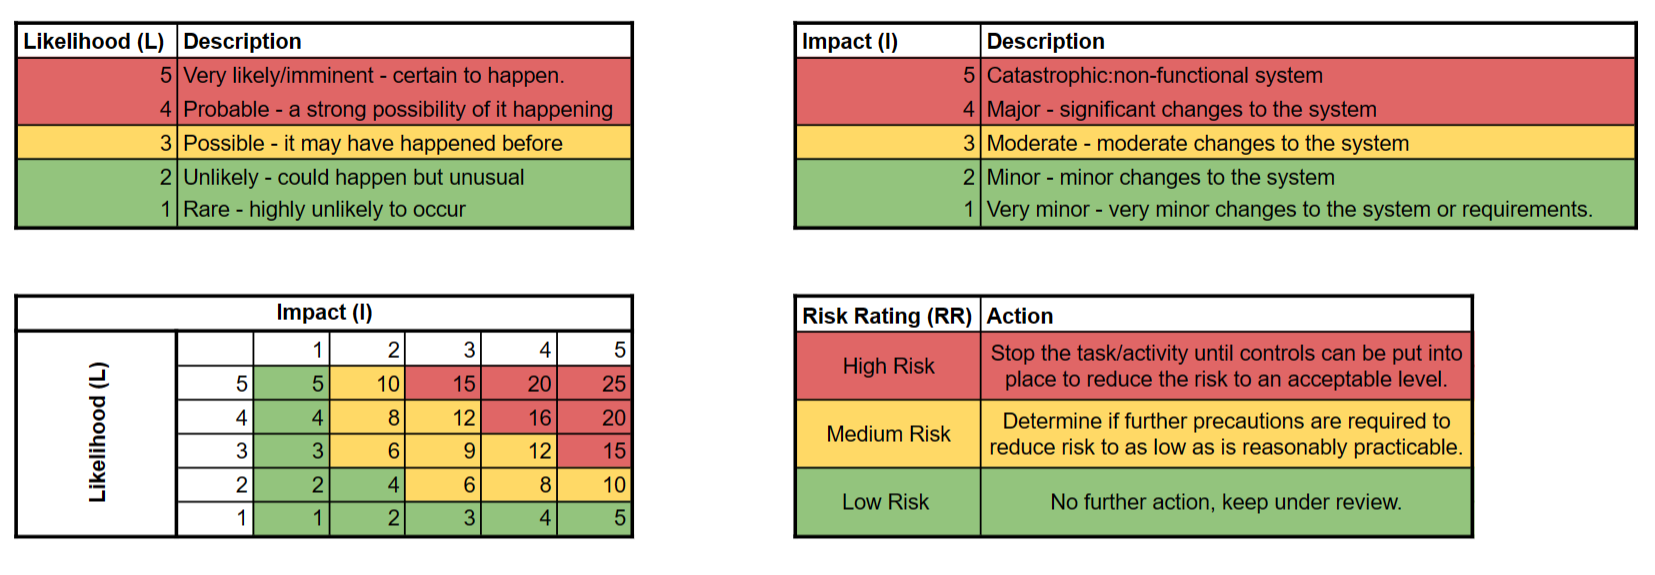
\includegraphics[width=1\linewidth]{images/ktrr.png}
    \caption{Key to Risk Rating}
    \label{fig:ktrr}
\end{figure}

\begin{figure}
    \centering
    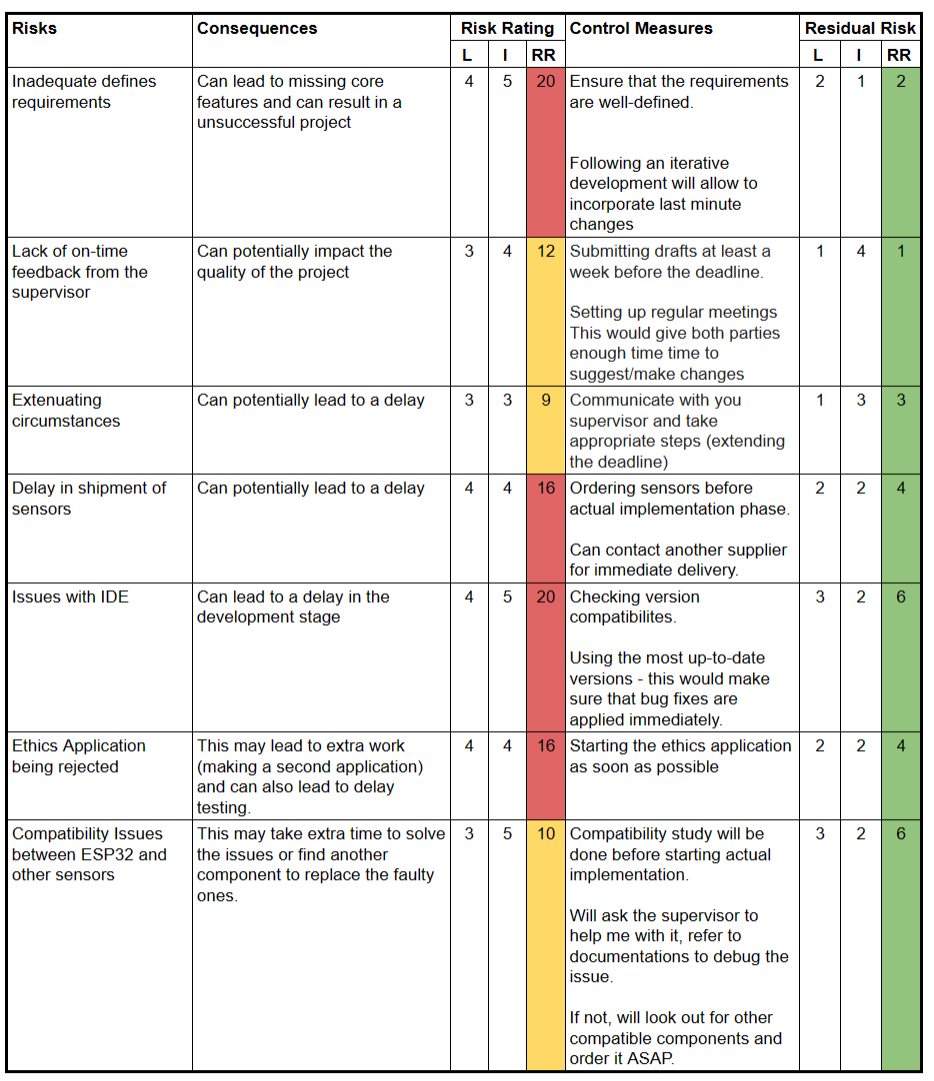
\includegraphics[width=1\linewidth]{images/rr.png}
    \caption{Risk Register}
    \label{fig:rr}
\end{figure}

\newpage
\section{Evaluation}
To ensure the robustness, reliability, and effectiveness of the Smart Patch and the dashboard, a comprehensive testing and quality assurance process will be implemented throughout the implementation and testing stage of the project:
\begin{itemize}
    \item \textbf{Unit tests:} Conducted to validate the correctness of individual components and the functionality of the Smart Patch and dashboard.
    \item \textbf{Integration testing:} Conducted to verify the seamless integration of components and modules within the Smart Patch and the dashboard.
    \item \textbf{System testing:} Conducted to assess the overall functionality and the performance of the integrated Smart Patch and the dashboard.
    \item \textbf{Acceptance Testing:} Covering all user stories to ensure that the system meets user requirements.
    \item \textbf{Manual testing:} For features that cannot be adequately tested using the above tests.
\end{itemize} 
A systematic evaluation of legal and ethical considerations will also take place:
\begin{enumerate}
    \item \textbf{Legal considerations:} Medical Regulations outlined by MHRA and GDPR guidelines will be followed (see \textbf{Appendix \ref{app:legal}}).
    \item \textbf{Ethical considerations:} Guidelines provided by the University of Sheffield will be followed, and an ethics application will be made if the project starts to use real human health data other than the developers' data (see \textbf{Appendix \ref{app:ethical}}).
\end{enumerate}


